\documentclass[12pt]{article}

\usepackage{amsmath}
\usepackage{amsthm}
\usepackage{amsfonts}
\usepackage{amssymb,amsfonts,amsxtra}         
\usepackage{epstopdf}
\usepackage{float}
\usepackage{subfigure}
\usepackage{epstopdf}
\usepackage{todonotes}
\usepackage{caption}
\usepackage{gensymb}
\usepackage{tikz}
\usepackage{hyperref}
\usepackage[capitalise]{cleveref}
\crefname{equation}{Eqn}{Eqns}
\crefname{subsection}{subsection}{subsections}
\crefname{figure}{Fig.}{Figs}
\usepackage{csquotes}
\usepackage{epigraph}
\usepackage{geometry}
\usepackage{pdflscape}
\usepackage[all]{nowidow}

\graphicspath{Figs/}

\usepackage{draftwatermark}
% \SetWatermarkLightness{0.8}
\SetWatermarkScale{4}

\begin{document}

\title{Kirigami Curvature DRAFT}
\author{S.R. Wilson \\ K.A. Seffen}
\date{\today}
\maketitle

\section*{Abstract}

Kirigami design differs from the well-known \textit{origami} by allowing cuts and material removal in a physical sheet in addition to folding. This work explores the use of kirigami as a basis for transforming  flat sheets into 3D shapes. By formulating the principles of kirigami with basic topology and differential geometry, a framework is developed for transforming a sheet between flat and curved configurations by through a ``suturing'' process. We demonstrate this process by designing and analyzing the pure kirigami unit cell. We find that this unit cell is a type of plane symmetric, 6R mechanical linkage. We analyze the kinematics of this linkage and illustrate one possible tessellation. We expect this system to find applications in morphing structures and robotics where transitions between curvature states are desired.


\begin{enumerate}
  \item intro\\ 
    \begin{enumerate}
      \item prior lit\\
      \item goals\\ 
    \end{enumerate}
  \item topology\\
    euler\\
    gauss bonnet \\
  \item geometry\\ 
    single hex unit \\ 
    hex tessellation \\ 
  \item future work 
    single curvature \\ 
\end{enumerate} 


%%%%%%%%%%
\section{Gauss-Bonnet Theorem}
%%%%%%%%%%
Topological principles, however, are not concerned with physical materials: ``rubber-sheet geometry'' is just that-- abstractions of objects in any dimension without resistance to large in-plane deformations. In order to move one rung down the ladder of abstraction, we seek a connection between the three-dimensional geometry of perforated sheets and their topology. This link is given by the Gauss-Bonnet Theorem, stated as
%
\begin{equation}
\int_{S}\!K\,\mathrm{d}A + \int_{\delta{S}}\!k_g\,\mathrm{d}s = 2\pi\chi.
\label{GBT1}
\end{equation}
%
$K$ is the Gaussian curvature within the surface, $S$, and $k_g$ is the geodesic curvature integrated over line elements, $ds$, along the boundary, $\delta{S}$, of S \cite{Knill2011}. This curvature computation is equated to the topological invariant $\chi$ from \cref{eq:euler}. This form of the theorem applies to orientable, compact objects-- conditions our kirigami structures must obey. This is an astounding result in differential geometry, a commandment for how objects must obey their topological invariant whilst undergoing deformation. A fundamental intuition of Gaussian curvature is essential for understanding the importance of morphing kirigami structures. Rather than merely changing the shape of an object, we can completely change its structural properties. For the perforated disc from \cref{euler}, we can insert \cref{eq:perfdisc} into \cref{GBT1} to yield 
%
\begin{equation}
\int_{S}\!K\,\mathrm{d}A + \int_{\delta{S}}\!k_g\,\mathrm{d}s = 2\pi(1-g).
\label{eq:GBT}
\end{equation}
%
Thus, we have a relationship between the number of kirigami cuts in our general surface, and how the curvature along the boundaries and within the sheet must reflect the homotopic change when a hole is closed. For brevity, we can rewrite \cref{eq:GBT} as 
%
\begin{equation}
\tau + \gamma = 2\pi(1-g)
\label{GBTshort}
\end{equation}
%
for use in subsequent discussion. For a closed surface without boundary, $\gamma$ will remain exactly 0. For a kirigami cell each hole will add an additional boundary, and the material will always contain an external boundary with changing geodesic curvature to reflect the opening or closing of holes as shown in \cref{paper_hole}. Thus, changing $g$ will manifest itself in a change in $\tau$ and $\gamma$.
%
\begin{figure}
    \centering
    \begin{subfigure}[b]{0.2\textwidth}
        \includegraphics[angle=-90,width=\textwidth]{paper_flat}
        \caption{Top view, open}
        \label{paper_flat}
    \end{subfigure}
    ~ %~, \quad, \qquad, \hfill etc. 
    \begin{subfigure}[b]{0.3\textwidth}
        \includegraphics[width=\textwidth]{paper_side}
        \caption{Side view, closed}
        \label{paper_side}
    \end{subfigure}
    ~ %\quad, \qquad, \hfill etc. 
    \begin{subfigure}[b]{0.2\textwidth}
        \includegraphics[width=\textwidth]{paper_top}
        \caption{Top view, closed}
        \label{paper_top}
    \end{subfigure}
    \caption{Thin sheet with a hole in open and closed configurations. This is the basic building block of a kirigami sheet transforming between two and three dimensions. In the closed configuration, the sheet's external boundary must accommodate the change in genus $g$ of the sheet.}\label{paper_hole}
\end{figure}
%%%%%%%%
\section{Discrete Gauss Bonnet Theorem}
%%%%%%%%
In this study, we focus on objects that can be modeled as polyhedral sheets with rigid, planar facets. To better understand the shape of general kirigami structures, we can develop a discrete form of \cref{eq:GBT} which is more efficient in computing the discrete curvature of polyhedral vertices. In its discrete form, we use angle measures and sums as opposed to integrals. We prove their equivalence and show in detail how they are used. 
%
\begin{figure}[htbp]
\begin{center}
\includegraphics[width=.7\textwidth]{gauss_map}
\caption{$(a)$ Non-developable vertex, $v$, with angle defect, $d(v)$, positive curvature and facet angles $\mu$. $(b)$ The spherical map of the vertex. The defect of the vertex is shown as the area, $d(v)$, of the spherical quadrilateral with interior angles $\rho$. The facets $A$ and $B$ map to vertices on the spherical polygon.}
\label{2Droof}
\end{center}
\end{figure}
%
%\begin{figure}[htbp]
%\begin{center}
%\includegraphics[width=\textwidth/3]{3Droof}
%\caption{Non-developable vertex and its gauss map.}
%\label{3Droof}
%\end{center}
%\end{figure}
%
For a discrete polyhedral surface, $S$, with boundary $\delta{S}$ composed of $n$ geodesics each of curvature $k_g$, it is straightforward to show 
%
\begin{equation}
\sum_{i=1}^{n}\int_{\delta{S_i}}\!k_g\,\mathrm{d}s = 0
\end{equation}
%
for each boundary edge $\delta{S}_i$. These edges are straight line segments (edges) with geodesic curvature 0. The boundary curvature is defined by the turning, or exterior, angles at the edge vertices, $\mu_{ext}$, where 
%
\begin{equation}
\mu_{ext}(v) =  \pi - \sum_{i}\mu_i
\label{descartes}
\end{equation}
%
for each $v\in\delta{S}$ where $i$ facets converge. The Gauss-Bonnet Theorem for a polyhedral surface composed of planar facets can be rewritten as  
%
\begin{equation}
\int_{\delta{A}}\!K\,\mathrm{d}A + \sum_{v\in\delta{S}}\mu_{ext} = 2\pi(1-g). 
\label{eq:GBT_turn}
\end{equation}
%
It can be shown that the Gaussian curvature concentrated at an interior polyhedral vertex $v$ is exactly $d$, the angle defect of that vertex \cite{calladine1989}. Since we restrict all facets to be rigid and planar for our kirigami, the integral of the Gaussian curvature over the surface is equal to the sum of the interior angle defects and each vertex defect is equal to the solid angle, $A$, subtended by a Gaussian spherical map of that vertex where
%
\begin{equation}
A = (2-n)\pi + \sum_{i=1}^{n}\rho_i.
\end{equation}
%
$\rho_i$ is the interior angle of the $i^{th}$ vertex of the spherical $n$-gon. It is trivial to show that $\mu_i$, the interior angle of the $i^{th}$ facet at polyhedral vertex $v$, is equivalent to $\pi-\rho_i$ making the angle defect, $d$, of that vertex 
%
\begin{equation}
d(v) = 2\pi - \sum_{i=1}^{n}\!\mu_i.
\end{equation}
\label{eq:defect}
%
The Gauss-Bonnet Theorem can thus be rewritten in discrete form as 
%
\begin{equation}
\sum_{v\in{S_{int}}} d(v) + \sum_{v\in\delta{S}}\mu_{ext}(v) = 2\pi(1-g) 
\label{GBTdiscrete}
\end{equation}
%
for a polyhedral surface, $S$, with interior $S_{int}$ and boundary $\delta{S}$. The parameters used in this derivation are shown in \cref{2Droof}. A similar analysis has been employed in computational geometry as a straightforward method of calculating discrete curvature for a polyhedral mesh \cite{Alboul2005}. We use this framework to explore the curvature of our kirigami unit cell. By constructing a series of Gauss maps, it becomes clear how the curvature of the surface changes throughout its transformation, and provides insight for how kirigami cells might be tessellated to form a globally curved shape. An important definition to state here is ``developable'', in terms of a surface. A developable polyhedral surface contains no vertices with nonzero discrete Gaussian curvature. To flatten a non-developable surface, some tear or cut must be made within the surface. Note that a fold is developable, and thus a vertex through which a single fold passes has exactly zero curvature. 
%%%%%%%
\section{Polyhedral Unfolding} 
%%%%%%%
We define \textit{pure kirigami} as the removal of material within the boundary of a finite sheet, and note that we subsequently use the term \textit{kirigami} to mean this construction. What, then, are the limits of kirigami? While fold lines are prescribed within the sheet to allow for mobility, what collection of non-developable vertices can be created to produce a globally curved kirigami structure? This problem falls under a niche category of origami engineering known as polyhedral unfolding, a graph theory topic in disguise. We investigate several key results in that field to mathematically define kirigami and build a vocabulary to better understand the geometric constraints involved. 

A graph is a collection of edges and vertices; a path is an ordered traversal of vertices on a graph through its edges; a cycle is a path that returns to its starting point. A tree is a graph with no cycles, and a forest is a disjoint collection of trees. Removing a  single edge from a tree results in a forest. A cutting graph, or cutting, is a collection of edges on a simply connected polyhedral surface or closed polyhedron that separates faces of that surface or polyhedron.  We seek cuttings that result in connected, flattened polyhedral surfaces called unfoldings. Specifically, we require unfoldings to not contain overlaps. Given a polyhedral surface, we can show that any unfolding is a forest, and that the cutting must traverse all vertices with nonzero curvature. By contradiction, if the cutting has a cycle, the unfolding will be disjointed. We want to retain the connectedness of our polyhedron in order to manufacture shapes from single sheets. Of course every polyhedral sheet has a trivial cycle along its boundary vertices, thus we exclude this case. If the cutting in question did not traverse all vertices with nonzero curvature, the faces joined by these vertices would not be flattenable. Thus, every nonzero curvature vertex must be included in the cutting. 
%
\begin{figure}[htbp]
\begin{center}
\includegraphics[width=\textwidth]{unfolding}
\caption{Statement of the general problem. $(a)$ A single, fictitious kirigami cell in some folded and cut configuration. $(b)$ Given a cutting forest, we seek a flattened kirigami geometry. }
\label{unfolding}
\end{center}
\end{figure}
%

The flattened polyhedral surface need not be simply connected, thus the cutting need not be a tree. As shown in \cref{unfolding}, a pure kirigami cell is a counterexample for this assumption. It is through connections of this type of component that we wish to create a global kirigami structure unfolded by a cutting forest. It has been proven that the requirement for this construction is nonconvexity \cite{Bern2003}. We digress here to briefly define convexity with effort to do justice to the field of convex polytopes. 
%
\begin{displayquote}\textit{A set $K$ of $\mathbb{R}^n$ is convex if, for each pair of distinct points $a$, $b$ in $K$, the closed segment with endpoints $a$ and $b$ is contained within $K$} \cite{Grunbaum2003}. \end{displayquote}
%
Another measure of convexity is the existence of ``saddle corners'', or vertices of negative discrete Gaussian curvature \cite{Orland1965}. 

Thus, for a closed, convex polyhedron, we know that, generally, the cutting must be a forest, and the connected graph condition of the cutting stems from the convexity condition. Assuming the cutting were a forest, one can imagine a closed contour on the polyhedron's surface, across its faces, that encloses one of the forest's trees entirely, avoiding any and all vertices of the polyhedron. When the cutting is made, this contour must unfold and flatten with the polyhedron meaning the sum of its turning angle, $\tau$ from \cref{GBTshort}, must equal $2\pi$. From the closed condition, the left-hand side of \cref{GBTshort} must be $2\pi$. Due to the convexity condition, $\gamma$ must be greater than or equal to zero (in the flattened state). However, since the contour must enclose at least one vertex of the polyhedron and the convexity condition enforces positive curvature on these vertices, $\gamma$ must be strictly greater than zero. Since $\tau$ must be less than $2\pi$ to comply with \cref{GBTshort}, the polyhedron cannot flatten. Thus, the cutting of a convex polyhedron must be a tree. Note that every negative curvature vertex must be connected to two cut edges, as a single cut would allow the faces of that vertex to overlap by its angle surplus. With these definitions and propositions defined, we apply this manner of thinking to explore what is possible for pure kirigami constructions. 
%
\section{Curvature of Kirigami Sheets}
\label{kiricurvature}

We would like to create kirigami structures with nonzero global curvature, an open polyhedron with some net angle defect, for double curvature is useful in creating shell structures with high strength to weight ratio such as spherical caps and saddles. This leads us to a question: does a polyhedral surface of some nonzero global curvature have a cutting that does not include any boundary vertices? In essence, we seek the existence of a non-developable structure with a cutting forest. We impose neither the convexity nor the closed condition on this structure, only that it has some nonzero net Gaussian curvature, no overlaps in the flattened state, and a disjoint cut tree. These are the requirements of a kirigami sheet in the language of graphs. We seek a flat sheet that can transform into a polyhedral shell or saddle by hole closures.   

A kirigami object, by our definition, is a polyhedral sheet with a cutting forest that does not include any boundary vertices. For a kirigami object with net nonzero Gaussian curvature, every interior vertex would need to have nonzero curvature. Thus, every vertex would need to be traversed by a cutting forest. For the pure kirigami unit, we use the simplest hole, the rhombus cut, as shown in \cref{unfolding}$(a)$. This unit creates three vertices, one of negative curvature and two of positive curvature. As the hole is closed, the curvature of the internal boundary in the flat configuration must shift to the outer boundary in the closed configuration. In order to create a global sheet through the addition of these kirigami units, the boundary vertices of adjacent cells are connected. In order to retain the disjoint cutting, the boundary vertices must combine to form vertices with zero curvature. Since every interior vertex in a doubly-curved surface must have nonzero curvature vertices, this construction contradicts the constraints imposed by the disjoint cutting forest. In order to create doubly-curved kirigami, the boundary vertices of the sheet must be contained by the cutting or the sheet will not be developable. Stated formally, all bounded polyhedral surfaces with disjoint cut trees which disassemble their non-developable vertices have net-zero global curvature. Thus, pure kirigami can not be used to construct bounded polyhedral surfaces with double curvature. This does not mean that we cannot created singly curved or ruled surfaces using pure kirigami, which provides a rich design space. We explore this space in detail in \cref{sq_rhomb_jelly} and \cref{octopus}. 


%%%%%%%%%%%%
\section{Introduction}
%%%%%%%%%%%%

\normalsize

% What is the problem and why is it interesting?
% Who are the main contributors?
% What did they do?
% What novel thing will you reveal? 

%why is this a good idea? why do we need this? 

%BACKGROUND 

Kirigami, the art of cutting paper, has recently emerged as an alternative to origami for manufacturing three-dimensional (3D) geometries from two dimensions (2D). While origami has drawbacks such as excess material and intricate folds, kirigami techniques circumvent these difficulties by removing excess material and producing objects with simple folds. Information for 3D shapes is programmed into 2D sheets through the geometry of cuts. The principles underpinning these cuts are an active topic of research, and open questions remain, such as generalized cutting rules that will allow embedding of the sheet in three dimensions \cite{Castle2014}. 

%GOAL 

This work is motivated by the increasing demand for responsive architectures--- interactive objects that respond to their environment. Research in this mode has presented shape-changing surfaces for aerodynamic designs, solar panels, and robotics \cite{Silverberg2014,Shim2012}. This work explores kirigami as a modular framework for transformable surface architecture. 
%STATE OF THE ART 
So-called ``pluripotent" materials have been explored to produce out-of-plane geometry from kirigami, where the distribution of cuts made in a sheet are limited to a hexagonal graph and its triangular dual \cite{Sussman2015}. Rules are devised and experiments approximate curvature through the use of basic geometric building blocks. The result is a height map where the achievable gradient is limited by the size of the chosen unit cell. Similar schemes have been explored on the nano-scale using graphene \cite{Blees2015}. 

Morphing structure design is rooted in repeating unit cell constructions. The geometry of the unit cell is analyzed and exploited through tessellation, such as the Miura-Ori geometry \cite{Silverberg2014,Schenk2013,Cheung2014,Chen2015}. The generalized problem of foldable sheets has been solved algorithmically, analytically, and computationally \cite{Demaine2007,Schief2008,Tachi2009a}. In robotics, the mathematical principles of folding have been applied to produce actuated structures \cite{Onal2011,Hawkes2010,Gilpin2010}. In the generalized schemes, each polygonal element of the sheet is thought to be rigid or to allow bending of the first order \cite{Schenk2010}. 

%VISION OF THE FUTURE

This work rebuilds the foundations of kirigami from topological principles to its geometric implications, and results in the design and analysis of a kirigami unit cell. Links are drawn between kirigami and overconstrained linkages, and this similarity is employed to determine tessellation rules for multiple degree-of-freedom kirigami networks. We envision a reconfigurable surface composed of kirigami units that is able to change between a variety of global mode shapes. We hope for this work to elucidate the principles of morphing kirigami design and to find a variety of applications. 

%%%%%%%%%%%%%%%%%
\thispagestyle{fancy}
\lhead{}
\chead{\textcolor[rgb]{0.5,0.5,0.5}{\textit{Proceedings of the IASS Annual Symposium 2016}\\\textit{Spatial Structures in the 21st Century}}}
\rhead{}
\cfoot{\thepage}
\lfoot{}
\rfoot{}
%%%%%%%%%%%%%%%%%


%%%%%%%%%%%
\section{Unit Cell}
%%%%%%%%%%%
%this is our case study, the unit we designed for the purpose of pluripotent sheet 

Cutting a disc from a thin sheet and joining the edges of the hole together produces a minimal surface containing a saddle and two peaks \cite{Guven2012}. Discretizing the disc into a rhombus results in the simplest hole that can be completely closed along straight edges. This is a form of the square lattice kirigami shown in \cref{fig:protounits}. With the removal of two fold lines, we obtain a single degree of freedom mechanism containing a rhomboidal hole, as shown in \cref{fig:unitcell}. We first apply the discrete Gauss-Bonnet theorem to the vertices of the unit cell in the open configuration and the closed configuration. As the topology is fixed, we analyze the geometry of the cell using the vector parameterization shown in \cref{fig:unitcell}.

\begin{figure}[htbp]
\begin{center}
\includegraphics[width=6cm]{figures/protounits.png}
\caption{Basic square lattice kirigami. (a) Flat, unfolded annulus state. (b) Transition state. (c) Sutured disc state with hole fully closed. }
\label{fig:protounits}
\end{center}
\end{figure}

\begin{figure}[htbp]
\begin{center}
\includegraphics[width=12cm]{figures/unitcell.png}
\caption{(a) Geometric parameterization of a one degree-of-freedom kirigami unit cell in its planar state. Vectors labeled $k$ are fold lines; those labeled $d$ are hole edges. (b) Rendering of the unit cell in a partially folded configuration. The origin (of the coordinates shown in red) is placed in the same position as in the parametric analysis.}
\label{fig:unitcell}
\end{center}
\end{figure}

%\begin{figure}[htbp]
%\begin{center}
%\includegraphics[width=8cm]{figures/render.png}
%\caption{A rendering of the unit cell in a partially folded configuration. The origin is placed in the same position as in the parametric analysis.}
%\label{fig:render}
%\end{center}
%\end{figure}

\begin{figure}[htbp]
\begin{center}
\includegraphics[width=10cm]{figures/gaussmaptotal.png}
\caption{Two extreme states of the unit cell from \cref{fig:unitcell}. (a) The open planar state shows the unique interior and exterior vertex angles. (b) The closed configuration in plan view shows the contours used to produce Gauss maps. The green and blue contours yield the positive and negative Gauss maps for individual vertices, respectively, while the red contour yields the gauss map of the interior of the unit cell in its closed configuration. These maps are shown in \cref{fig:gaussmaps,fig:fullmap}, respectively.}
\label{fig:gaussmaptotal}
\end{center}
\end{figure}

\begin{figure}[htbp]
\begin{center}
\includegraphics[width=\textwidth]{figures/gaussmaps.png}
\caption{(a) One of two angular defect vertices in the interior of the closed until cell and its corresponding Gauss map. (b) The center saddle vertex of the closed unit cell and its corresponding Gauss map. }
\label{fig:gaussmaps}
\end{center}
\end{figure}

\begin{figure}[htbp]
\begin{center}
\includegraphics[width=\textwidth/2]{figures/gaussmapbig.png}
\caption{Gauss map of the three interior vertices in the closed configuration of the unit cell. The total solid angle as a sum of each signed area is zero; thus, the interior holds no net Gaussian curvature as expected.}
\label{fig:fullmap}
\end{center}
\end{figure}

In the open configuration, summing the interior angles and the exterior turning angles of \cref{fig:gaussmaptotal} yields

\begin{equation}
[2(2\alpha) + 2(\pi - 2\alpha)] + [4(\pi - \alpha_{ext,2} + 2(\pi - \alpha_{ext,1})] = 2\pi\chi = 0
\end{equation}

where the exterior angles are:

\begin{equation}
\alpha_{ext,1} = \pi +2\alpha, \hspace{.5cm} \alpha_{ext,2} = \frac{3\pi}{2}-\alpha
\end{equation}

and $\chi$ is $0$ for an annulus; in the closed configuration $\chi$ is $1$. The angular defect computation becomes a calculation of spherical polygon area, denoted $A_{quad}$ and $A_{tri}$ for the area of a spherical quadrilateral and triangle, respectively: 

\begin{equation}
A_{quad} = \sum_{i}^{3}\!\alpha_i - 2\pi = 2(\pi - 2\beta) + 2(2\alpha + 2\beta) - 2\pi =  4\alpha 
\end{equation}

\begin{equation}
A_{tri} = \sum_{i}^{3}\!\alpha_i - \pi = 2(\,\frac{\pi}{2}-\beta)+(2\alpha+2\alpha) =  2\alpha. 
\end{equation}

Thus, the angular defect 

\begin{equation}
d(v) = 2(2\alpha) - 4\alpha = 0 
\end{equation}

where the center solid angle is negative due to its clockwise direction shown in \cref{fig:gaussmaptotal}. We see that the curvature, upon closing a cell, shifts to the exterior vertices and sums to $2\pi$. By tessellating unit cells, we can take advantage of this curvature shift to construct a modular sheet with global shape by the combination of changing geometries. 


%\section{Parameterization}

%(INCOMPLETE)
%
%%
%The Rodrigues rotation formula is a straightforward method of rotating a 3-vector $\mathbf{v}$ about an axis $\mathbf{k}$ by angle $\theta$ according to the right-hand rule:
%
%\begin{equation}
%\mathbf{v}_{\mathrm{rot}} = \mathbf{v}\cos{\theta}  + (\mathbf{k}\times\mathbf{v})\sin{\theta} + \mathbf{k}(\mathbf{k}\cdot\mathbf{v})(1 - \cos{\theta}).
%\end{equation}
%
%Using the Rodrigues equation, we find relationships between $L$, $H$, and $W$ shown in \cref{fig:shape}.
%
%When the unit cell is in the closed position, we find a relationship between the dihedral and sector angles
%
%\begin{equation}
%\begin{split}
%\sin(\alpha) + 2\cos^2(\beta)\sin(\alpha)\cos(\rho_{2,closed}) + 2\cos(\alpha)\cos(\beta)\sin(\beta)\cos(\rho_{2,closed}) - \sin(\alpha + 2\beta) = 0
%\end{split} 
%\end{equation}
%
%EQUATIONS FOR L W and H 

%\begin{equation}
%W = 2*abs(l*abs(sin(alpha) - cos(beta)^2*sin(alpha) + cos(beta)^2*sin(alpha)*cos(rho2) - cos(alpha)*cos(beta)*sin(beta) + cos(alpha)*cos(beta)*sin(beta)*cos(rho2)) + b*abs(cos(beta)^2*cos(rho2) - cos(beta)^2 + 1))
%\end{equation}
%
%
%\begin{equation}
%L = abs(abs(l*cos(alpha)*cos(rho1) + l*cos(beta)*sin(alpha)*sin(rho1)*sin(rho2) + l*cos(beta)*sin(beta)*(cos(rho1) - 1)*(cos(rho2) - 1)*(sin(alpha) - cos(beta)^2*sin(alpha) + cos(beta)^2*sin(alpha)*cos(rho2) + cos(alpha)*cos(beta)*sin(beta) - cos(alpha)*cos(beta)*sin(beta)*cos(rho2))) + abs(l*cos(alpha)*cos(rho2) + l*cos(alpha)*cos(beta)^2 - l*cos(beta)*sin(alpha)*sin(beta) - l*cos(alpha)*cos(beta)^2*cos(rho2) + l*cos(beta)*sin(alpha)*sin(beta)*cos(rho2)) + a*abs(cos(beta)*(cos(rho1)*cos(rho2) - cos(rho2) - 2*cos(rho1) - 3*cos(beta)^2 + 2*cos(beta)^4 + 3*cos(beta)^2*cos(rho1) + 5*cos(beta)^2*cos(rho2) - 2*cos(beta)^4*cos(rho1) - 4*cos(beta)^4*cos(rho2) - 2*cos(beta)^2*cos(rho2)^2 + 2*cos(beta)^4*cos(rho2)^2 + sin(beta)*sin(rho1)*sin(rho2) - 5*cos(beta)^2*cos(rho1)*cos(rho2) + 4*cos(beta)^4*cos(rho1)*cos(rho2) + 2*cos(beta)^2*cos(rho1)*cos(rho2)^2 - 2*cos(beta)^4*cos(rho1)*cos(rho2)^2 + 1)) + a*abs(cos(beta)))
%\end{equation}

%\begin{equation}
%H = abs(sin(rho2)*(l*sin(alpha + beta) + b*cos(beta)))
%\end{equation}
%
%
%EQUATIONS FOR EQUAL HINGES 
%
%\begin{figure}[htbp]
%\begin{center}
%\includegraphics[width=8cm]{figures/facet.png}
%\caption{default}
%\label{default}
%\end{center}
%\end{figure}
%
%\begin{figure}[htbp]
%\begin{center}
%\includegraphics[width=8cm]{figures/shape.png}
%\caption{Side and front view of the unit cell with parametric values shown.}
%\label{fig:shape}
%\end{center}
%\end{figure}
%
%\begin{equation}
%1 - \frac{1}{\sin(\alpha)} + \frac{\sin(\beta)}{\sin(\alpha)} = \frac{\cos(\alpha)}{\cos(\beta)} - 1
%\end{equation}
%
%\begin{figure}[htbp]
%\begin{center}
%\includegraphics[width=8cm]{figures/hinges.png}
%\caption{default}
%\label{hinges}
%\end{center}
%\end{figure}
%
%POISSON RATIOS

%%%%%%%%%%%
\section{6R Linkage}
%%%%%%%%%%%
%this is an interesting analogue to our problem, that we can use to tell the kinematics of the linkage 

We identify an analogous linkage of the unit cell which is a special case of the 6R Bricard linkage \cite{Chen2005}, drawn in \cref{fig:linkage}. A linkage with $n$ bodies connected by $g$ joints where joint $i$ allows $f_i$ freedoms is said to have a difference between mobility $m$ and states of self-stress $s$ according to the generalized Kutzbach criterion \cite{Guest2005}

\begin{equation}
m - s = 6(n-1) - 6g + \sum_{i=1}^{g}\!f_i.
\end{equation}

The unit cell is deemed to have equal mobility and states of self-stress with six bodies connected by six single degree of freedom joints. By inspection, the linkage has zero states of self stress and must have zero mobility according to the generalized Kutzbach. However, the linkage has multiple mobility modes due to geometric symmetry. This overconstrained linkage is ideal for the purpose of a multiple degree of freedom sheet because it allows a single actuator to change the shape of a cell while influencing the global structure. To analyze the kinematics, we use a modified form of the Denavit-Hartenberg parameters \cite{Belcastro2002}. Because all hinges lie in the plane for a kirigami sheet, we do not require homogenous coordinates to compute offset axes. All adjacent fold axes meet at a point, requiring just rotations around two axes, as shown in \cref{fig:linkage}. Thus, each composite transformation is a 3x3 orthogonal matrix 

%With an extended symmetry analysis, we recover symmetric and antisymmetric mobilities for the linkage. 

%symmetry table for point group representation analysis 
%\begin{table}[htp]
%\caption{default}
%\begin{center}
%\begin{tabular}{|c|c|}
%SYMMETRY & \\
%POINT & GROUPS \\ 
%\end{tabular}
%\end{center}
%\label{default}
%\end{table}


\begin{equation}
T_{ij} = 
\begin{bmatrix}
\cos\mathrm{\theta_i} & - \sin\mathrm{\theta_i} & 0\\ 
\cos\mathrm{\alpha_i} \sin\mathrm{\theta_i} & \cos\mathrm{\theta_i} \cos\mathrm{\alpha_i} & - \sin\mathrm{\alpha_i}\\     
\sin\mathrm{\alpha_i} \sin\mathrm{\theta_i} & \cos\mathrm{\theta_i} \sin\mathrm{\alpha_i} & \cos\mathrm{\alpha_i} 
\end{bmatrix}
\label{eq:rotation}
\end{equation}

where $T_{ij}$ is the transformation from link $i$ to link $j$ shown in \cref{fig:linkage}. Using symmetry, we set two opposing composite transformations equal to find a closure condition for the linkage 

\begin{equation}
[T_{12}][T_{23}][T_{34}] = [T_{61}]^T[T_{56}]^T[T_{45}]^T
\label{eq:closure}
\end{equation}

%alpha is the sector angle, theta is fold angle, rho is the param 

where the sector angles $\alpha$ and fold angles $\theta$ about the $x$ and $z$ axes shown in \cref{fig:linkage} adhere to the following relationships 

\begin{equation}
\begin{split}
\alpha_1 = \alpha_2 = \alpha_4 = \alpha_5 &= \frac{\pi}{2}-\beta; ~~ \alpha_3 = \alpha_4 = 2\,\beta \\  
 \theta_1 = \theta_3 = \theta_4 = \theta_6 &= \rho_2; ~~ \theta_2 = \theta_5 = \rho_1.
\end{split}
\end{equation}

\begin{figure}[htbp]
\begin{center}
\includegraphics[width=6cm]{figures/linkage.png}
\caption{The 6R linkage analog to the kirigami unit cell, shown in its inital planar configuration. Coordinate transformations are made from joint 1 to joint 4 in both directions around the loop to generate a closure condition based on a modified Denavit-Hartenburg protocol.}
\label{fig:linkage}
\end{center}
\end{figure}

By analyzing the closure condition in \cref{eq:closure}, we identify a periodic isosurface which visualizes the continuous motions of the linkage as a function of $\beta$, the geometric hinge angle, governed by 

\begin{equation}
\begin{split}
\sin\rho_1\sin\rho_2 + \sin^3\beta 
+ \cos2\beta\sin\beta\cos\rho_2 
+ \sin^3\beta\cos\rho_1\cos^2\rho_2 & \\
+ \cos2\beta\sin\beta\cos\rho_1\cos\rho_2 
- \cos^2\beta\sin\beta\cos\rho_1 
- \sin\beta\cos\rho_1\sin\rho_2^2  & \\ 
- 2\cos^2\beta\sin\rho_1\sin\rho_2 
- \cos^2\beta\sin\beta\cos^2\rho_2 
- 2\sin^2\beta\cos\rho_2\sin\rho_1\sin\rho_2 &= 0.
\end{split}
\end{equation}

The isosurface informs the configuration of each individual unit cell by providing an input-output relationship. Given a geometric angle $\beta$ and one hinge angle, we can solve for the third unknown hinge angle which completely describes the state of the cell at any given geometry and configuration. This will inform a network of cells by providing the ability to describe the configuration of any cell within a tessellation. We plot this isosurface and numerically find the value for $\beta$ for the minimum area closure loop, shown in \cref{fig:isosurface}. If we assume the flexural hinges in the kirigami cell to act as linear-elastic beams for a first approximation, strain energy scales linearly with hinge width. Thus, the minimum area kinematic loop is thought to correspond to the least energy geometry, the geometric design with the least amount of motion to achieve continuous transformation of the linkage. 

\begin{figure}[htbp]
\begin{center}
\includegraphics[width=7cm]{figures/isosurface.png}
\caption{The isosurface is shown in red, which provides all continuous solutions given a geometric quantity $\beta$ for the linkage as a function of $\rho_1$ and $\rho_2$ shown in \cref{fig:unitcell}. The minimum area solution for $\beta$ is found and plotted as a contour in blue.}
\label{fig:isosurface}
\end{center}
\end{figure}

%\begin{figure}[htbp]
%\begin{center}
%\includegraphics[width=12cm]{figures/isocontour.png}
%\caption{default}
%\label{fig:isocontour}
%\end{center}
%\end{figure}

%%%%%%%%%%%%%%
\thispagestyle{fancy}
\lhead{}
\chead{\textcolor[rgb]{0.5,0.5,0.5}{\textit{Proceedings of the IASS Annual Symposium 2016}\\\textit{Spatial Structures in the 21st Century}}}
\rhead{}
\cfoot{\thepage}
\lfoot{}
\rfoot{}
%%%%%%%%%%%%%%

%%%%%%%%%%%%
\section{Tessellation}
%%%%%%%%%%%%
%this is a stab at the big goal 

We describe a preliminary tessellation structure of the unit cell in one and two dimensions. The one dimensional network of cells is shown in various configurations in \cref{fig:1Dtessellation}. By actuating $n$ cells independently, we have $2^n$ possible configurations in one dimension. For a surface that is able to morph into a plethora of shapes, we seek a method of linking 1D strands together. In \cref{fig:2Dtessellation}, we offer one method of tessellating in two dimensions that involves snubbing the hexagonal units into octagons and rotating the fold lines of the original unit by $\frac{\pi}{2}$. This tessellation shows promise in creating a sheet with $n$ degrees of freedom from $n$ unit cells. However, this pattern creates a pattern of rectangular cuts that affect the shear strength of the sheet. This may be mitigated by altering the geometry of the unit cells, and is being explored. 

\begin{figure}[htbp]
\begin{center}
\includegraphics[width=12cm]{figures/1Dtessellation.png}
\caption{(a) For a one dimensional tessellation with $n$ units, we have $2^n$ configurations, with five shown. By adjusting the geometry of the unit, we can create tessellations in a range of shapes. (b) Rendering of one configuration. (c) Physical prototype. }
\label{fig:1Dtessellation}
\end{center}
\end{figure}

The current geometric and linkage analysis informs only the unit cell kinematics and geometry. In order to design a network of kirigami linkages, we must take a combinatorial approach to the problem to efficiently generate a list of geometrically plausible networks. It is nontrivial to extend a 1D tessellation into 2D due to self intersection and non-developability constraints. We can then experiment with tessellations to understand their transformations by combining the constituent unit cell kinematics. In order to devise a set of feasible tessellations, we are currently exploring methods of abstracting unit cell connections in order to systematically formulate the problem. This combinatorial formulation remains our principle challenge. 

\begin{figure}[htbp]
\begin{center}
\includegraphics[width=12cm]{figures/2Dtessellation.png}
\caption{A possible tessellation in two dimensions. All units are closed in the same sense here, approximating a doubly curved sheet. The tessellation uses two unique unit cells shown in red and blue, with hinge lines rotated by $\frac{\pi}{2}$. (a) Side view of the tessellation. (b) Isometric view with the unfolded configuration. (c) Physical model.}
\label{fig:2Dtessellation}
\end{center}
\end{figure}


%1D TESSELLATION IN RHINO -- make a circle!!!!! 

%\section{Protoyping}       
%       
%       materials 
%       tooling 
%       mechanical design 
%           hinges 
%           geometry 
%   actuation 
%       EPM actuators 
%       preliminary design 
%       mock-up cad/graphic 

\section{Conclusion}
%this is the vision we have, what we would like to achieve, end-to-end, why this is a good start 

We present preliminary work towards a new approach for kirigami engineering utilizing unit cell construction. Using basic differential geometry, we illustrate how a shift in curvature for a polyhedral unit cell occurs when changing homotopy groups. We outline a framework for creating surfaces exploiting this curvature shift that are able to morph in a general manner using modular units. By creating a network of $n$ continuously kinematic linkages, we propose an $n$-degree of freedom surface for unit-by-unit, distributed actuation to produce an array of shapes. By characterizing the motion of the unit cell, we can combine cells to describe the shape of the actuated network. 

This method of shape change is likened to muscle architecture, and could show promise in the generation of undulatory motion. Using a regular pattern of kirigami cuts with irregular closure patterns over the sheet, this scheme is the foundation for a distributed actuation of a patterned sheet in order to produce a variety of shapes. The authors are working to build a working prototype to physically realize the design and identify new problems.

%the point is that you have this really cool new geometric system
%your 6 bar element
%and you want to explore what it can and can't do
%so a regular set of kirigami cuts but irregular closure
%and you think it offers the possibility for distributed actuation
%and you've characterised the motion using whatever schemes
%kirigami linkage networks
%especially because they might be easier to construct than bar networks
\newpage
\section*{References}

%\bibliographystyle{plain} %sorted by list in bib file 
\bibliographystyle{unsrt} %sorted in citation order 
%\bibliography{Bib/PaperBib,references}
\bibliography{biblio}


%What is topology? Its history. Why is it useful to an engineer?

%Introduce the concept of a Euler characteristic and genus in order to set up the discussion of the GBT in the next section 

%Show how to apply basic topological principles to find the Euler characteristic of a kirigami sheet.
%
%GBT relates the intrinsic geometry of the genus/euler characteristic with the extrinsic geometry of curvature in the embedding. 
%We introduce the Gauss Bonnet Theorem as a link between topology and the case study geometries we are concerned with. Why did we settle on these geometries? We start with the simple square lattice and make punctures. We distort this lattice into rhomboidal tessellations and into nonregular tessellations, such as the jellyfish and octopus tessellations. \\
%
%immersions in $R^3$? minimal surface of a glued hole in a sheet...?\\
%%%	
%�although homeomorphic surfaces have the same euler characteristic the converse is false, as shown by X(T) = X(K) but T=/= K.� p.65\\
%
%�for compact surfaces M1 and M2, X(M1M2) = X(M1) + X(M2) - 2�\\
%
%homeomorphic iff X(M1) = X(M2) and they are both orientable or both non-orientable \\
%
%**we are essentially crafting a plane model of an orientable surface, and the engineering trick is the glueing of this surface \\
%
%a complex is a polygonalization of a plane model � different from a pattern \\
%topology is somewhat of a dead end � we can characterize the surface given a number of holes, and show that it changes homotopy groups, but we are simply confirming gauss bonnet.\\
%	can we show topological equivalence to another problem? \\
%		why? \\
%
%what is interesting is writing the surface as a plane model, and thinking about the problem algebraically� \\
%
%GBT: Any orientable compact surface without boundary is topologically equivalent to a sphere with some handles attached\\ 
%
%
%recast the problem into an algebraic topology question? 
%	use the method of plane diagrams to come up with an algebra problem taking into account the connections of holes 
%		�> this doesn�t exactly help, but could be of use to someone smarter than I am? \\ 
%		--> redraw the terrains as plane models, describe the issue algebraically from there?\\ 
%
%Lemma 3. Any cutting of a polyhedron P is a forest, and spans every non-boundary vertex of P that has nonzero curvature.
%	a cutting is a flattening of the polyhedra
%Proof. If a cutting contained a cycle, having positive area both interior and exterior to the cycle, then the resulting unfolding would be disconnected, a contradiction. 
%(Above we excluded the possibility of the cutting containing a cycle on the boundary of an open polyhedron P.) 
%	an open polyhedron obviously has a trivial cycle on the boundary 
%If the cutting did not contain a particular (non-boundary) point with nonzero curvature, neighborhoods of that point could not be flattened without overlap. 
%	nonzero curvature vertices must be traversed to flatten them
%tree - acyclic graph 
%forest - collection of trees
%removing an edge from a tree makes a forest 
%
%A common assumption is that an unfolding must be a simple polygon, which implies that a cutting of a closed polyhedron must furthermore be a (connected) tree; see, e.g., [8,9,22]. 
%	the cutting is one big tree 
%Without this restriction, in most cases, a cutting of a closed polyhedron is a tree, but in fact this is not always the case. Fig. 2 illustrates a basic construction for separating off a connected component of the cutting. We could add cuts to connect the inner tree to the rest of the forest, but these extra cuts are unnecessary. Using this construction, we can build a polyhedron and a cutting having arbitrarily many connected components, by connecting a series of the constructions in Fig. 2 in a �dented barrel� shape, and then capping the ends. Together with Joseph O�Rourke (personal communication, July 2001), we have proved that such examples require nonconvexity: 
%Lemma 4. Any cutting of a convex closed polyhedron is a tree.
%	this is a very strong condition. closed, first of all, and convex. what is the definition of convexity? 
%		
%Proof. By Lemma 3, the cutting is a forest. Suppose for contradiction that the forest has multiple connected components. Then there is a closed path p on the surface of the polyhedron that avoids all cuts and strictly encloses a connected component of the cutting. In particular, p avoids all vertices of the polyhedron. Let ? denote the total turn angle along the path p. Because p avoids vertices, it
%unfolds to a connected (uncut) closed path in the planar layout; thus, ? = 2�. Because the polyhedron is homeomorphic to a sphere, the Gauss�Bonnet theorem [6, pp. 215�217] applied to p says that
%? +? =2� where ? is the curvature enclosed by p. By convexity, ? ?0. Further, p encloses a connected component of the cutting, which consists of at least one vertex of the polyhedron, so ?>0. Therefore, ?<2�, contradicting that p could lay out flat in the plane.
%
%Lemma 5. If v is a vertex of a polyhedron P with negative curvature, then any cutting of P must include more than one cut incident to v.
%Proof. Suppose some cutting C includes only a single cut incident to v.Let N be P ?B,where B is a small ball around v. Neighborhood N unfolds to a small disk that self-overlaps by precisely the absolute
%value of the curvature of v. 
%
%This requires looking at the curvatures of the nodes in the constituent components. 
%
%convex polytopes (from \cite{Grunbaum2003})
%A convex polytope, like any closed convex subset of Rn, is homeomorphic to a closed ball.[7] Let m denote the dimension of the polytope. If the polytope is full-dimensional, then m = n. The convex polytope therefore is an m-dimensional manifold with boundary, its Euler characteristic is 1, and its fundamental group is trivial. The boundary of the convex polytope is homeomorphic to an (m ? 1)-sphere. The boundary's Euler characteristic is 0 for even m and 2 for odd m. The boundary may also be regarded as a tessellation of (m ? 1)-dimensional spherical space � i.e. as a spherical tiling.

%first we design a different cell, a few different ones
%we look at its mobility and symmetry 
%we look at its geometry and curvature
%we look at its angle relationships as a linkage
%then we try to tessellate it to make something interesting. 
%
We experimented with unit cells analogous to 8R linkages in \cref{sq_rhomb_jelly}. For a sheet with embedded actuators, it is difficult to control two degrees of freedom per unit cell when one of the degrees of freedom is nonplanar. By removing two fold lines, we change the unit cell topology, decrease the degrees of freedom, and create an overconstrained 6R kirigami linkage containing a rhombus hole. We name this cell the ``octopus''' cell due to its form and motion as shown in \cref{unitcell}. 
%
%MOBILITY + SYMMETRY 
%%%%%%%%%%%%%
\section{Mobility and Symmetry}
\label{octosymmetry}
%%%%%%%%%%%%%
%
We begin an analysis of the octopus cell by investigating its mobility. We identify a special case of the general 6R Bricard linkage analogous to the unit cell drawn in \cref{linkage}. The unit cell is deemed to have equal mobility and states of self-stress with six bodies connected by six single degree of freedom joints. By inspection, the linkage has zero states of self stress and must have zero mobility according to the generalized Kutzbach criterion. However, the linkage has multiple mobility modes due to geometric symmetry. This overconstrained linkage is ideal for the purpose of a morphing sheet because it allows a single actuator to change the shape of a cell while influencing the global shape of the structure. 
%
\begin{figure}[htbp]
\begin{center}
\includegraphics[width=0.8\textwidth]{unitcell.png}
\caption{(a) Geometric parameterization of a one degree-of-freedom kirigami unit cell in its planar state. Vectors labeled $k$ are fold lines; those labeled $d$ are hole edges. (b) Rendering of the unit cell in a partially folded configuration. The origin (of the coordinates shown in red) is placed in the same position as in the parametric analysis.}
\label{unitcell}
\end{center}
\end{figure}
%
This cell has two symmetry planes; we can create a contact polyhedron $C$ shown in \cref{octopus_contact}$(a)$ to apply the symmetry-extended mobility formulae described in \cref{symmetry_formula}. By inspection the cell has three folding modes: two symmetric and one antisymmetric shown in \cref{mobilitymodes}. We seek these of these modes through representation calculations. For the doubly symmetric cell, the lowest point group symmetry is $C_s$, with one symmetry plane. The character table for this group is supplied in \cref{Cs_table}. Using the $C_s$ character table, we calculate the representations in \cref{Cs_rep}. The identity operation, $E$, does not displace any nodes, thus the difference between the mechanism and self stress representations is zero, while the symmetry plane provides a difference of two. Since the cell is known to have the same number of mechanisms and self-stresses, due to symmetry there exist two mechanisms and two corresponding self-stresses.  
%
\begin{figure}[htbp]
\begin{center}
\includegraphics[width=.8\textwidth]{octopus_contact}
\caption{The contact polyhedra, $C$, for symmetry calculations. $(a)$ C for the doubly symmetric linkage. $(b)$ C for the singly symmetric linkage.}
\label{octopus_contact}
\end{center}
\end{figure}
%
\begin{figure}[htbp]
\begin{center}
\includegraphics[width=.8\textwidth]{octocellmodes}
\caption{Paper prototype showing three mobility modes of the octopus cell. $(a)$ Primary symmetric mode. $(b)$ Secondary symmetric mode. $(c)$ Antisymmetric mode.}
\label{mobilitymodes}
\end{center}
\end{figure}
%
\begin{table}[htp]
\caption{The $C_s$ character table.}
\begin{center}
\def\arraystretch{1.3}
\begin{tabular}{P{1.5cm}|P{1.5cm}|P{1.5cm}}
$C_s$ & E & $\sigma$  \\ \hline
A' & 1 & 1 \\ \hline
A'' & 1 & -1 \\ 
\end{tabular}
\end{center}
\label{Cs_table}
\end{table}
%
\begin{table}[htbp]
\caption{The symmetry calculation for the symmetric octopus cell.}
\begin{center}
\def\arraystretch{1.3}
\begin{tabular}{c|c|c}
$\Gamma(m) - \Gamma(s)$ = & E & $\sigma$ \\ \hline
$\Gamma(v,C)$ & 6 & 0 \\ \hline
$\times$ $\Gamma_T$ + $\Gamma_R$ & $\times$ 6 & $\times$ 0 \\ \hline
- $\Gamma_{\parallel}(e,C)$ & -6 & -(-2) \\ \hline
$\times$ $\Gamma_T$ + $\Gamma_R$ & $\times$ 6 & $\times$ 0 \\ \hline
-$\Gamma_T$ + $\Gamma_R$ & -6 & 0 \\ \hline
+ $\Gamma_f$ & 6 & 2 \\ \hline
= & 0 & 2 \\ 
\end{tabular}
\end{center}
\label{Cs_rep}
\end{table}
%
From the character table, these mechanisms must belong to a symmetric mode, $A'$, and an antisymmetric mode, $A''$, where
%
\begin{equation}
\Gamma(m) - \Gamma(s) = A'' - A'. 
\end{equation}
%
Since the representations must be positive, the mechanism here is due to a symmetry and an antisymmetry, $A'' + A'$ and the self stresses are $A' + A'$. This means the representation calculation shows one symmetric mechanisms and one antisymmetric, with two symmetric self stresses. We can imagine these self stresses being due to hinge misalignment in a translational or rotational sense. This calculation is repeated to explore the mechanisms of the singly-symmetric cell, which is of interest for the design of curved sheets. The contact polyhedron is shown in \cref{octopus_contact}$(b)$. The singly-symmetric cell's plane of symmetry, $\sigma$, does not pass through any hinge lines. The representation calculation is shown in \cref{anti_rep} and results in no mechanisms since all hinge lines are permuted by the reflection operation. 
%
\begin{table}[htbp]
\caption{The symmetry calculation for the asymmetric octopus cell.}
\begin{center}
\def\arraystretch{1.3}
\begin{tabular}{c|c|c}
$\Gamma(m)$ - $\Gamma(s)$ = & E & $\sigma$ \\ \hline
$\Gamma(v,C)$ & 6 & 2 \\ \hline
$\times$ $\Gamma_T$ + $\Gamma_R$ & $\times$ 6 & $\times$ 0 \\ \hline
- $\Gamma_{\parallel}(e,C)$ & -6 & 0 \\ \hline
$\times$ $\Gamma_T$ + $\Gamma_R$ & $\times$ 6 & $\times$ 0 \\ \hline
- \{$\Gamma_T$ + $\Gamma_R$\}  & -6 & 0 \\ \hline
+ $\Gamma_f$ & 6 & 0 \\ \hline
= & 0 & 0 \\ 
\end{tabular}
\end{center}
\label{anti_rep}
\end{table}
%
The resulting representation equation reveals 
%
\begin{equation}
\Gamma(m) - \Gamma(s) = 0 \times A' + 0 \times A''.
\end{equation}
%
Thus, there are no symmetric or antisymmetric modes. This is surprising given the ability of the singly symmetric cell to close as shown in \cref{antisymmobility}. Note that the symmetry-extended mobility rule is a necessary but not sufficient condition for mobility, thus there can still exist finite mechanisms in spite of the formula's outcome \cite{Fowler2000}. In this case, a close inspection of the cell reveals slight compliance in the facets. The magnitude of the necessary compliance to mobilize the singly-symmetric kirigami loop is discussed in \cref{vectors}. Given the lowest symmetry group, $C_s$, for the cell, there is a descent in symmetry between differing planes, $\sigma$, which allows for the mobility of the linkage. This fact is useful in the parametric design of repeating lattice structures, as altering the symmetry of neighboring cells has a profound impact on the mobility of the global network. A simple conclusion we can draw from this analysis is to design symmetry through hinge lines to allow mobility. This simple rule could play a powerful in the design of future kirigami tessellations. 
%
%GEOMETRY
%%%%%%%%
\section{Geometry}
%%%%%%%%
To explore the consequences of the fold line removal, we investigate the discrete curvature of the unit cell vertices by applying the discrete Gauss-Bonnet theorem in the open and closed configurations.
%
\begin{figure}[htbp]
\begin{center}
\includegraphics[width=0.7\textwidth]{gaussmaptotal.png}
\caption{Open and closed states of the unit cell from \cref{unitcell}. (a) The open, planar configuration shows the unique interior and exterior vertex angles. (b) The closed configuration shows the contours used to produce Gauss maps. The green and blue contours yield the positive and negative Gauss maps for individual vertices, respectively, while the red contour yields the gauss map of the interior of the unit cell in its closed configuration. These maps are shown in \cref{gaussmaps,fullmap}, respectively.}
\label{gaussmaptotal}
\end{center}
\end{figure}
%
\begin{figure}[htbp]
\begin{center}
\includegraphics[width=\textwidth]{gaussmaps.png}
\caption{(a) One of two angular defect vertices in the interior of the closed until cell and its corresponding Gauss map. (b) The center saddle vertex of the closed unit cell and its corresponding Gauss map.}
\label{gaussmaps}
\end{center}
\end{figure}
%
\begin{figure}[htbp]
\begin{center}
\includegraphics[width=\textwidth/2]{gaussmapbig.png}
\caption{Gauss map of the three interior vertices in the closed configuration of the unit cell. The total solid angle as a sum of each signed area is zero; thus, the interior holds no net Gaussian curvature as expected.}
\label{fullmap}
\end{center}
\end{figure}
%
In the open configuration, summing the interior rhombus angles and the exterior turning angles of \cref{gaussmaptotal} yields
%
\begin{equation}
[2({2\alpha}) + 2(\pi - 2\alpha)] + [4(\pi - \alpha_{ext,2} + 2(\pi - \alpha_{ext,1})] = 2\pi\chi = 0
\end{equation}
%
where the exterior angles are:
%
\begin{equation}
\alpha_{ext,1} = \pi +2\alpha, \hspace{.5cm} \alpha_{ext,2} = \frac{3\pi}{2}-\alpha.
\end{equation}
%
In the open configuration, the cell is an annulus and $\chi$ is $0$. In the cell's closed configuration, $\chi$ becomes $1$. The angular defect computation becomes a calculation of spherical polygon area, denoted $A_{quad}$ and $A_{tri}$ for the area of a unit spherical quadrilateral and triangle, respectively: 
%
\begin{equation}
A_{\textrm{quad}} = \sum_{i}^{3}\!\alpha_i - 2\pi = 2(\pi - 2\beta) + 2(2\alpha + 2\beta) - 2\pi =  4\alpha 
\end{equation}
%
\begin{equation}
A_{\textrm{tri}} = \sum_{i}^{3}\!\alpha_i - \pi = 2(\,\frac{\pi}{2}-\beta)+(2\alpha+2\alpha) =  2\alpha. 
\end{equation}
%
Thus, the angular defect is 
%
\begin{equation}
d(v) = 2({2\alpha}) - 4\alpha = 0 
\end{equation}
%
where the center solid angle is negative due to its clockwise direction shown in \cref{gaussmaptotal}. The curvature, upon closing a cell, shifts to the exterior vertices and sums to $2\pi$. This is a continuous phenomenon; the spherical map changes throughout the cell's closing. By tessellating unit cells, we can take advantage of this curvature shift to construct a modular sheet with global shape through the combination of changing geometries. By imagining the spherical polygons created throughout the cell's motion, this discrete curvature approach gives us an intuitive sense of the kinematics in terms of angle defects and spherical maps to design networks of unit cells. We now turn to a vector parameterization of the cell in order to calculate the shape of a cell with a given geometry. 
%
%VECTORS
%%%%%%%%%%%%%%%%%%%
\subsection{Vector Parameterization}
\label{vectors}
%%%%%%%%%%%%%%%%%%%
%
% width, heigh, length 
% actuator throw 
% compliance of antisymmetric 
%
%numerical check:   
%for beta = 30
%alpha = 15
%rho2 = 54.6? 
%solve for:
%rho1 = 28.67
%kcross = 86.4? 
%
As the topology is fixed, we analyze the geometry of the cell using the vector parameterization shown in \cref{unitcell}. Using vector analysis, we can produce geometric relationships between the cell's components for use in structural design. By placing vectors along hinge lines and the hole edges, we can keep track of the facet positions throughout the cell's motion. The Rodrigues rotation formula is a straightforward method of rotating a general vector $\mathbf{v}$ about an axis $\mathbf{k}$ by angle $\theta$ according to the right-hand rule \cite{rodrigues}
%
\begin{equation}
\mathbf{v}_{\mathrm{rot}} = \mathbf{v}\cos{\theta}  + (\mathbf{k}\times\mathbf{v})\sin{\theta} + \mathbf{k}(\mathbf{k}\cdot\mathbf{v})(1 - \cos{\theta}).
\end{equation}
%
%
\begin{figure}[htbp]
\begin{center}
\includegraphics[width=.8\textwidth]{shape.png}
\caption{Side and front view of the unit cell with parametric values shown.}
\label{shape}
\end{center}
\end{figure}
%
When the unit cell is in the closed configuration, we find a relationship between the dihedral angles, $\rho_i$ and sector angles, $2\beta$ and $\frac{\pi}{2}-\beta$, for one half of a cell where $\rho_2$ is a function of $\alpha$ and $\beta$  
%
\begin{equation}
\cos(\rho_{2,\textrm{closed}}) = \frac{\sin(\alpha + 2\beta) - \sin{\alpha}}{2\sin{\alpha}\cos^2{\beta} + 2\cos{\alpha}\cos{\beta}\sin{\beta}}.
%cos(rho2) = (sin(alpha + 2*beta) - sin(alpha))/(2*sin(alpha)*cos(beta)^2 + 2*cos(alpha)*cos(beta)*sin(beta))
%f(rho2closed) = f(alpha,beta)
%plug this into kdot equation for middle vector angle 
\label{closed}
\end{equation}
%
For the closed cell, we find the angle, $\phi_w$ between the normalized vectors $\hat{k_1}$ and $\hat{k_2}$ that span the middle plane
%
\begin{equation}
\begin{aligned}
\hat{k_1} \cdot \hat{k_2} &= \cos{\phi_w}\\ 
 &=  4\cos^2{\beta} - 2\cos^4{\beta} - 4\cos^2{\beta}\cos{\rho_{2,\textrm{closed}}} \\ 
 &+ 4\cos^4{\beta}\cos{\rho_{2,\textrm{closed}}} - 2\cos^4{\beta}\cos^2{\rho_{2,\textrm{closed}}} - 1
%kdot = 4*cos(beta)^2 - 2*cos(beta)^4 - 4*cos(beta)^2*cos(rho2) + 4*cos(beta)^4*cos(rho2) - 2*cos(beta)^4*cos(rho2)^2 - 1 
%dot product of the two k vectors in the middle plane 
%angle = arccos(kdot)
\label{kdot}
\end{aligned}
\end{equation}
%
where $\rho_{2,\textrm{closed}}$ is the dihedral angle in the closed configuration. Substituting \cref{closed} into \cref{kdot}, we find $\phi_w$ as a function on $\alpha$ and $\beta$ only 
%
\begin{equation}
 \cos{\phi_w}  = -\frac{\cos{2\beta} - \cos{2\alpha} + \sin{2\alpha}\sin{2\beta}}{\cos(2\alpha + 2\beta) - 1}. 
%kdot_alpha  = -(cos(2*beta) - cos(2*alpha) + sin(2*alpha)*sin(2*beta))/(cos(2*alpha + 2*beta) - 1)
%checked, works!
\label{kdotsimp}
\end{equation}
%
For each half of the unit cell to match, the angle, $\phi_w$ spanned in the middle plane must match. For the singly-symmetric cell, this condition is violated. From \cref{kdotsimp}, we see that changing $\alpha$ while holding $\beta$ constant will lead to a twisting of the cell's facets on the order of the change in $\alpha$ due to the change in $\phi_w$. Changing the length of one side of the unit cell changes $\cos{\alpha}$, stretching one side of the cell and removing the second plane of symmetry, leading to twisting of the facets. By keeping the antisymmetric change small, we can limit the facet twisting to a trivial level. While the symmetry formula yields zero mobility for the singly-symmetric unit cell, through experimentation we find very small compliance in the cell when it is moved into the closed position shown in \cref{antisymmobility}. With apt material selection and geometric design, it may prove useful for morphing structures despite its necessary deformation. 
%
%%%%%%%%
%EQUATIONS FOR LENGTH WIDTH and HEIGHT  
%%%%%%%%
%
By attaching a local coordinate system shown in \cref{unitcell}, we find relationships for $H$ and $W$ shown in \cref{shape} throughout the cell's motion where 
%
\begin{equation}
\begin{aligned}
H =  & || \sin{\rho_2}(l\sin(\alpha + \beta) + b\cos{\beta}) || \\ 
& \\ 
%abs(sin(rho2)*(l*sin(alpha + beta) + b*cos(beta))) 
W =  & 2l ||\sin{\alpha} - \cos^2{\beta}\sin{\alpha} + \cos^2{\beta}\sin{\alpha}\cos{\rho_2} \\
        & - \cos{\alpha}\cos{\beta}\sin{\beta} + \cos{\alpha}\cos{\beta}\sin{\beta}\cos{\rho_2} || \\ 
        & + 2b || \cos^2{\beta}\cos{\rho_2} - \cos^2{\beta} + 1) || 
%2*abs(l*abs(sin(alpha) - cos(beta)^2*sin(alpha) + cos(beta)^2*sin(alpha)*cos(rho2) - cos(alpha)*cos(beta)*sin(beta) + cos(alpha)*cos(beta)*sin(beta)*cos(rho2)) + b*abs(cos(beta)^2*cos(rho2) - cos(beta)^2 + 1)).
\end{aligned}
\end{equation}
%
for the height and width, respectively, of the cell throughout its deployment. The middle plane spanned by the hinges $k_1$ and $k_4$ is described by the normal $\hat{n}$, shown in \cref{shape}. We find $\hat{n}$ using the cross product of $k_1$ and $k_2$ such that 
%
\begin{equation}
\renewcommand*{\arraystretch}{1.5}
\hat{n} = \begin{bmatrix} \frac{\sin{\beta}\sqrt{1 - \cos{\rho_2}}}{\sqrt{(\cos^2{\beta}\cos{\rho_2} - \cos^2{\beta} + 2)}} \\
- \frac{\sin{\rho_2}}{\sqrt{(1 - \cos{\rho_2})(\cos^2{\beta}\cos{\rho_2} - \cos^2{\beta} + 2)}} \\
0
\end{bmatrix}.
\end{equation}
%
We find a relationship for the middle plane angle, $\phi_s$, shown in \cref{shape} as a function of $\hat{n}$
%
%angle phi for the midplane 
\begin{equation}
\phi_s = \frac{\pi}{2} - \arccos(\hat{n}\cdot-\hat{y}). 
\end{equation}
%
where $\hat{y}$ is the unit vector in the $y$ coordinate direction. Computing this relationship for $\phi_s$ yields 
%
\begin{equation}
\cos(\phi_s) =  \frac{\sqrt{\frac{4\cos(2\alpha + 2\beta) - 4\cos{2\beta}}{\cos{2\alpha} - 2\cos{2\beta} + 2\cos(2\alpha + 2\beta) + \cos(2\alpha + 4\beta) - 2}}}{\sqrt{\frac{3\sin(\alpha + \beta) - \sin(\alpha - \beta)}{\sin(\alpha + \beta)}}\sqrt{\frac{\sin{\alpha}}{\sin{\alpha} + \sin(\alpha + 2\beta)}}}. 
\end{equation}
%
%LENGTH OF THE OCTOPUS CELL 
Using this relationship, we can find an expression for the length of the cell 
%
\begin{equation}
L = 2 R_z^{\phi_s}( ( |d_1| + |k_1| + |k_2| ) \ast \hat{y} )
%= abs(abs(l*cos(alpha)*cos(rho1) + l*cos(beta)*sin(alpha)*sin(rho1)*sin(rho2) + l*cos(beta)*sin(beta)*(cos(rho1) - 1)*(cos(rho2) - 1)*(sin(alpha) - cos(beta)^2*sin(alpha) + cos(beta)^2*sin(alpha)*cos(rho2) + cos(alpha)*cos(beta)*sin(beta) - cos(alpha)*cos(beta)*sin(beta)*cos(rho2))) + abs(l*cos(alpha)*cos(rho2) + l*cos(alpha)*cos(beta)^2 - l*cos(beta)*sin(alpha)*sin(beta) - l*cos(alpha)*cos(beta)^2*cos(rho2) + l*cos(beta)*sin(alpha)*sin(beta)*cos(rho2)) + a*abs(cos(beta)*(cos(rho1)*cos(rho2) - cos(rho2) - 2*cos(rho1) - 3*cos(beta)^2 + 2*cos(beta)^4 + 3*cos(beta)^2*cos(rho1) + 5*cos(beta)^2*cos(rho2) - 2*cos(beta)^4*cos(rho1) - 4*cos(beta)^4*cos(rho2) - 2*cos(beta)^2*cos(rho2)^2 + 2*cos(beta)^4*cos(rho2)^2 + sin(beta)*sin(rho1)*sin(rho2) - 5*cos(beta)^2*cos(rho1)*cos(rho2) + 4*cos(beta)^4*cos(rho1)*cos(rho2) + 2*cos(beta)^2*cos(rho1)*cos(rho2)^2 - 2*cos(beta)^4*cos(rho1)*cos(rho2)^2 + 1)) + a*abs(cos(beta)))
\end{equation}
%
where $R_z^{\phi_s}$ is a rotation around the $z$ axis by $\phi_z$ and $\ast$ is element-wise multiplication. We leave this expression in its symbolic form as the equations become quite long. The process to calculate these geometric relationships numerically is straightforward. 
%
%LINKAGE
%%%%%%%%%%%%%%%%%%%%%
\section{Linkage Analysis}
%%%%%%%%%%%%%%%%%%%%% 
%
To analyze the kinematics, we use a modified form of the Denavit-Hartenberg parameters \cite{Belcastro2002}. For the kirigami cell where the structure begins in a flat configuration where all adjacent fold axes meet at a point, the protocol outlined in \cref{dh_protocol} requires only rotations around two axes, as shown in \cref{linkage}, where the sector angles $\alpha$ and fold angles $\theta$ about the $x$ and $z$ axes shown in \cref{linkage} adhere to the following relationships 
%
\begin{table}[H]
\caption{Denavit-Hartenberg parameters for the general 6R kirigami linkage.}
\begin{center}
\begin{tabular}{c|c|c|c|c}
Link & $\alpha$ & $a$ & $\theta$ & $d$ \\ \hline 
1 & $\frac{\pi}{2}-\beta$ & 0 & $\rho_2$ & $d$ \\ \hline 
2 & $\frac{\pi}{2}-\beta$ & 0 & $\rho_1$ & 0 \\ \hline 
3 & $2\,\beta$ & 0 & $\rho_2$  & $d$ \\ \hline 
4 & $\frac{\pi}{2}-\beta$ & 0 & $\rho_2$  & $d$ \\ \hline 
5 & $\frac{\pi}{2}-\beta$ & 0 & $\rho_1$ & 0 \\ \hline 
6 & $2\,\beta$ & 0 & $\rho_2$  & $d$ \\ 
\end{tabular}
\end{center}
\label{dhparamtable}
\end{table}
To simplify the analysis we set $d$ to 0 for all links, effectively shrinking the rhombus hole to a point, converting the kirigami cell into a degree-6 origami vertex. This way we simplify our calculations to focus on the angle relationships, summarized as 
%
\begin{equation}
\begin{aligned}
\alpha_1 = \alpha_2 = \alpha_4 = \alpha_5 &= \frac{\pi}{2}-\beta, \alpha_3 = \alpha_6 = 2\,\beta \\  
a_i &= 0 \\ 
 \theta_1 = \theta_3 = \theta_4 = \theta_6 &= \rho_2, \theta_2 = \theta_5 = \rho_1 \\
 d_i &= 0 
\end{aligned}
\end{equation}
%
Compared to the Bricard linkages listed in \cref{BakerBricard}, the kirigami linkage is a type of plane-symmetric linkage as confirmed from the mobility approach in \cref{octosymmetry}. Using these parameters, we compute transformation matrices between each of the six coordinate systems. Our loop closure condition based on the $C_s$ symmetry of the cell, 
%
\begin{equation}
R_{12}R_{23} R_{34}  = R_{16}R_{65} R_{54}
\end{equation}
%
yields six equations where $R_{ij}$ is the transformation matrix from coordinate system $i$ to $j$. As there is one independent geometric parameter for the sector angles, $\beta$, and two parameters, $\rho_1$ and $\rho_2$, for the hinge angles, there is only one independent loop closure equation: 
%
\begin{equation}
\begin{split}
\centering 
\sin\rho_1\sin\rho_2 + \sin^3\beta 
& + \cos2\beta\sin\beta\cos\rho_2 \\ 
+ \sin^3\beta\cos\rho_1\cos^2\rho_2 
& + \cos2\beta\sin\beta\cos\rho_1\cos\rho_2 \\
&= \\
 \cos^2\beta\sin\beta\cos\rho_1 
& - \sin\beta\cos\rho_1\sin^2\rho_2 \\ 
- 2\cos^2\beta\sin\rho_1\sin\rho_2 
- \cos^2\beta\sin&\beta\cos^2\rho_2 
- 2\sin^2\beta\cos\rho_2\sin\rho_1\sin\rho_2.
\end{split}
\end{equation}
%
This relationship between the three independent angular parameters of the kirigami unit cell serves as an input-output relationship. By defining the geometry of the cell through $\beta$, we can solve for the unknown hinge angle given a certain configuration. This relationship can be plotted as an isosurface of possible configurations for the linkage as shown in \cref{isosurface}. The function is $2\pi$ periodic as we would expect, though for physical solutions we assume that $\rho_1$ is between $\frac{-\pi}{2}$ and 0, $\rho_2$ is between 0 and $\frac{\pi}{2}$, and $\beta$ is between 0 and $\frac{\pi}{4}$. The isosurface visualizes the solution space of these parameters. As we can see, there are solutions for all $\beta$ beginning from $(\rho_1,\rho_2) = (0,0)$ as well as a separate solution set beginning from $\beta = \frac{\pi}{4}$. By choosing two variables, we can numerically solve for the third, which allows us to completely characterize our unit cell in any geometry and configuration. For a given $\beta$, there exists a contour of solutions as a function of the kinematic variables, the kinematic path. 
%
%equation 4  (used to make the figures), independent equation 
%eqn4 = sin(rho1).*sin(rho2) + sin(beta).^3 + cos(2.*beta).*sin(beta).*cos(rho2) + sin(beta).^3.*cos(rho1).*cos(rho2).^2 + cos(2.*beta).*sin(beta).*cos(rho1).*cos(rho2) - ( cos(beta).^2.*sin(beta).*cos(rho1) + sin(beta).*cos(rho1).*sin(rho2).^2 + 2.*cos(beta).^2.*sin(rho1).*sin(rho2) + cos(beta).^2.*sin(beta).*cos(rho2).^2 + 2.*sin(beta).^2.*cos(rho2).*sin(rho1).*sin(rho2));
%all equations
%eqn1 = sin(beta).*sin(rho1) + sin(beta).^2.*sin(rho2) + cos(beta).^2.*cos(rho1).*sin(rho2) + cos(beta).^4.*cos(rho2).*sin(rho2) + cos(beta).^2.*sin(beta).*cos(rho2).*sin(rho1) - ( sin(beta).^3.*sin(rho1) + sin(beta).^4.*sin(rho2) + cos(beta).^4.*cos(rho1).*sin(rho2) + cos(beta).^2.*cos(rho1).*cos(rho2).*sin(rho2) + 2.*cos(beta).^2.*sin(beta).*cos(rho2).^2.*sin(rho1) + cos(beta).^2.*sin(beta).^2.*cos(rho1).*cos(rho2).*sin(rho2));
%eqn2 = cos(rho2).*sin(rho1) + sin(beta).^3.*sin(rho2) + sin(beta).^2.*sin(rho1).*sin(rho2).^2 + sin(beta).*cos(rho1).*sin(rho2) + cos(beta).^2.*sin(beta).*cos(rho2).*sin(rho2) - ( cos(rho2).*(cos(beta).^2.*sin(rho1) + sin(beta).^2.*cos(rho2).*sin(rho1) + sin(beta).*cos(rho1).*sin(rho2)) + cos(beta).^2.*sin(beta).*cos(rho1).*sin(rho2) + sin(beta).^3.*cos(rho1).*cos(rho2).*sin(rho2));
%eqn3 = sin(2.*rho2) + 4.*sin(rho2) + 4.*sin(beta).*sin(rho1) + 4.*cos(rho1).*sin(rho2) + 4.*cos(beta).^2.*cos(rho2).*sin(rho2) + 4.*sin(beta).*cos(rho2).*sin(rho1) + 4.*cos(beta).^2.*cos(rho1).*cos(rho2).*sin(rho2) - ( 2.*cos(rho2).*sin(rho2) + 4.*cos(beta).^2.*sin(rho2) + 4.*cos(beta).^2.*cos(rho1).*sin(rho2) + 8.*sin(beta).*cos(rho2).^2.*sin(rho1) + 8.*cos(rho1).*cos(rho2).*sin(rho2));
%eqn4 = sin(rho1).*sin(rho2) + sin(beta).^3 + cos(2.*beta).*sin(beta).*cos(rho2) + sin(beta).^3.*cos(rho1).*cos(rho2).^2 + cos(2.*beta).*sin(beta).*cos(rho1).*cos(rho2) - ( cos(beta).^2.*sin(beta).*cos(rho1) + sin(beta).*cos(rho1).*sin(rho2).^2 + 2.*cos(beta).^2.*sin(rho1).*sin(rho2) + cos(beta).^2.*sin(beta).*cos(rho2).^2 + 2.*sin(beta).^2.*cos(rho2).*sin(rho1).*sin(rho2));
%eqn5 = cos(rho2).*sin(rho1) + 2.*sin(beta).^3.*sin(rho2) + 2.*sin(beta).^2.*sin(rho1).*sin(rho2).^2 + sin(beta).*cos(rho1).*sin(rho2) + 2.*cos(beta).^2.*sin(beta).*cos(rho2).*sin(rho2) - ( cos(2.*beta).*cos(rho2).*sin(rho1) + 2.*sin(beta).^2.*cos(rho2).^2.*sin(rho1) + cos(2.*beta).*sin(beta).*cos(rho1).*sin(rho2) + 2.*sin(beta).^3.*cos(rho1).*cos(rho2).*sin(rho2) + 2.*sin(beta).*cos(rho1).*cos(rho2).*sin(rho2));
%eqn6 = sin(beta).*(cos(rho2) + 2.*cos(beta).^2 - 2.*cos(beta).^2.*cos(rho2) - 2) + 2.*sin(rho1).*sin(rho2).*(2.*cos(beta).^2 - 1) + 2.*cos(beta).^2.*sin(beta).*cos(rho1) + 2.*sin(beta).*cos(rho1).*sin(rho2).^2 + 2.*cos(beta).^2.*sin(beta).*cos(rho2).^2 + 4.*sin(beta).^2.*cos(rho2).*sin(rho1).*sin(rho2) - ( sin(beta).*cos(rho2).*(2.*cos(beta).^2 - 2.*cos(rho1) + 4.*cos(beta).^2.*cos(rho1) + 2.*sin(beta).^2.*cos(rho1).*cos(rho2) - 1));
%
%\begin{figure}[htbp]
%\begin{center}
%\includegraphics[width=6cm]{6Rlinkage.png}
%\caption{The 6R linkage analog to the kirigami unit cell, shown in its inital planar configuration. Coordinate transformations are made from joint 1 to joint 4 in both directions around the loop to generate a closure condition based on a modified Denavit-Hartenburg protocol.}
%\label{linkage}
%\end{center}
%\end{figure}
%
%\begin{figure}[htbp]
%\centering
%\includegraphics[width=.6\textwidth]{isosurface.png}
%\caption{Three views of the three-dimensional isosurface shown in blue, which provides all continuous solutions given a geometric quantity $\beta$ for the linkage as a function of $\rho_1$ and $\rho_2$. Contours on the surface shown in red.}
%\end{figure}
%
\begin{figure}[htbp]
\centering 
\begin{subfigure}[b]{.48\textwidth}
\includegraphics[width=\textwidth]{isosurface1.png}
\end{subfigure}
~
\begin{subfigure}[b]{0.48\textwidth}
\includegraphics[width=\textwidth]{isosurface3.png}
\end{subfigure}
\\
\begin{subfigure}[b]{0.65\textwidth}
\includegraphics[width=\textwidth]{isosurface2.png}
\end{subfigure}
\caption{Three views of the three-dimensional isosurface shown in blue, which provides all continuous solutions given a geometric quantity $\beta$ for the linkage as a function of $\rho_1$ and $\rho_2$. Contours on the surface are shown in red.}
\label{isosurface}
\end{figure}
%
% TESSELLATION 
%%%%%%%%%%%%%
\section{Octopus Networks}
%%%%%%%%%%%%%
%
Given a single degree of freedom unit cell, we explore tessellations of this cell, or linkage networks. Beginning in one dimension, we can tile the cells end-to-end to achieve an $n$ degree of freedom structure with $n$ connected cells. This structure can take $2^n$ configurations seeing as shown in \cref{1Dtessellation}. By snubbing the corners of the octopus cell, we can tile the octagons by rotating the fold lines of the original cell. This tessellation is one degree of freedom regardless of the number of cells in the network. The hinge lines provide constraints along each edge which sets the configuration of the neighboring cell. We note that given the additional, non-actuated ``holes'' in this octagonal tessellation, double curvature may be achieved using non-regular cells, as shown in \cref{2Dtessellation}. However, this is not ``pure'' kirigami as we have previously defined given the additional voids in the sheet. Utilizing the angle defined by the geometric parameters of the cell, we develop a ring structure of one degree of freedom which lifts out of plane upon closing the voids in the cells. The radius and height of this structure can be controlled simply by the geometry of the individual cells and the number included in the tessellation as shown in \cref{octoring}. 
%For a ring of 8 cells, we find the geometric parameters such that
%
% RING MATH FOR 8 CELLS 
%
%and for 16 cells 
%
%RING MATH FOR 16 CELLS. 
%
%
\begin{figure}[htbp]
\begin{center}
\includegraphics[width=\textwidth]{1Dtessellation.png}
\caption{(a) For a one dimensional tessellation with $n$ units, we have $2^n$ configurations, with five shown. By adjusting the geometry of the unit, we can create tessellations in a range of shapes. (b) Rendering of one configuration. (c) Physical prototype.}
\label{1Dtessellation}
\end{center}
\end{figure}
%
\begin{figure}[htbp]
\begin{center}
\includegraphics[width=.8\textwidth]{2Dtessellation.png}
\caption{A possible tessellation in two dimensions. All units are closed in the same sense here, approximating a doubly curved sheet. The tessellation uses two unique unit cells shown in red and blue, with hinge lines rotated by $\frac{\pi}{2}$. (a) Side view of the tessellation. (b) Isometric view with the unfolded configuration. (c) Physical model.}
\label{2Dtessellation}
\end{center}
\end{figure}
%
\begin{figure}[htbp]
\begin{center}
\includegraphics[width=.6\textwidth]{octoring}
\caption{$(a)$ Design for an 8 cell octopus ring. $(b)$ Design for a 16 cell octopus ring. $(c)$ 8 cell physical prototype. $(d)$ 16 cell physical prototype.}
\label{octoring}
\end{center}
\end{figure}
%
To test the feasibility of physical cells, we fabricate a unit cell from 3mm high-density polyethylene (HDPE) using a Roland MDX-40 micro-milling machine. The cell functions as expected with hinges of 1mm thickness. The physical cell is shown in the flat and deployed states in \cref{octoplastic}. For tessellations, a larger CNC machine could be used to produce a meter-scale tessellation in a short time. 
%   
\begin{figure}[htbp]
\begin{center}
\includegraphics[width=.8\textwidth]{plastic}
\caption{(a) Top view of the cell in the open configuration. (b) Side view of the cell in the closed configuration. (c) Top view of the cell in the closed configuration.}
\label{octoplastic}
\end{center}
\end{figure}
%
We wish to tessellate the 6R kirigami cell without the addition of extra holes as in the case of the 2D octagonal tessellation. To achieve this, we design a hexagonal cell able to tile without voids in singly symmetric and doubly symmetric versions as shown in \cref{hexcell} with labeled geometric parameters. We dub this cell the ``hexapus'' unit. The kinematics of this cell are identical to the octopus cell; only the geometry is slightly changed, and all of the previous analysis still applies. 
%
\begin{figure}[htbp]
\begin{center}
\includegraphics[width=.8\textwidth]{hexantisymcell}
\caption{Paper prototype of an singly-symmetric octopus cell. $(a)$ The open configurations. $(b)$ The mode due to geometric hinge alignment, without compliance. $(c)$ The closed, antisymmetric mode requiring facet compliance.}
\label{antisymmobility}
\end{center}
\end{figure}
%
\begin{figure}[htbp]
\begin{center}
\includegraphics[width=0.7\textwidth]{hexcell.png}
\caption{$(a)$ A hexagonal octopus cell with unequal side lengths and only one symmetry plane. $(b)$ A hexagonal unit cell with two symmetry planes.}
\label{hexcell}
\end{center}
\end{figure}
%
As shown in \cref{hexmodes}, the hexagonal tessellation is a one degree of freedom structure capable of transforming between flat and singly-curved structures. The stiffness of the cylindrical shell shown here is based from the non-developable vertices created during the hole gluing process. The radius and length of the cylinder can be altered by the size of the tessellation and the cells' geometric parameters. The internal shape of a tube with equal-sided hexagonal cells, where the internal cross section is a regular polygon of $n$ sides corresponding to a tessellation $n$ cells wide. The design parameter for a tessellation that closes exactly into a cylindrical structure is 
%
\begin{equation}
\cos(\frac{\pi(n - 2)}{n}) = -\frac{\cos{2\beta} - \cos{2\alpha} + \sin{2\alpha}\sin{2\beta}}{\cos(2\alpha + 2\beta) - 1}
\end{equation}
% 
invoking \cref{kdotsimp} and the interior angle formula for regular polygons. 
%
%HEX CYLINDER MATH -- how do I design a cylinder using these bricks? 
%RADIUS (closed)
%HEIGHT (closed) 
%LENGTH (open)
%WHAT ARE THE PARAMETERS OF THIS TUBE??? 
%
%\begin{figure}
%\begin{center}
%\includegraphics[width=.5\textwidth]{hexequaltess.png}
%\end{center}
%\caption{$(a)$ Design for a 2D tessellation of equal-sided hexagonal cells. $(b)$ 2D hexagonal tessellation in the flat state. $(c)$ 2D hexagonal tessellation in the tubular folded state.}
%\label{hextubeflat} 
%\end{figure}
%
\begin{figure}
\begin{center}
\includegraphics[width=\textwidth]{hextransform}
\end{center}
\caption{Design for a 2D tessellation of equal-sided hexagonal cells. $(a)$ The flat-folded state. $(b)$ Unfurled to the planar state. $(c)$ The partial closed folded state. $(d)$ The final, non-developable closed cylinder state.}
\label{hexmodes} 
\end{figure}    
%
We can use the hexapus cell to create ring structures in the same manner as the octopus cell. This manner of tessellation can be used to create conical structures as shown in \cref{hexring}. Note that this singly symmetric unit cell will include a small degree of compliance in order to transform its shape. 
%
\begin{figure}
\begin{center}
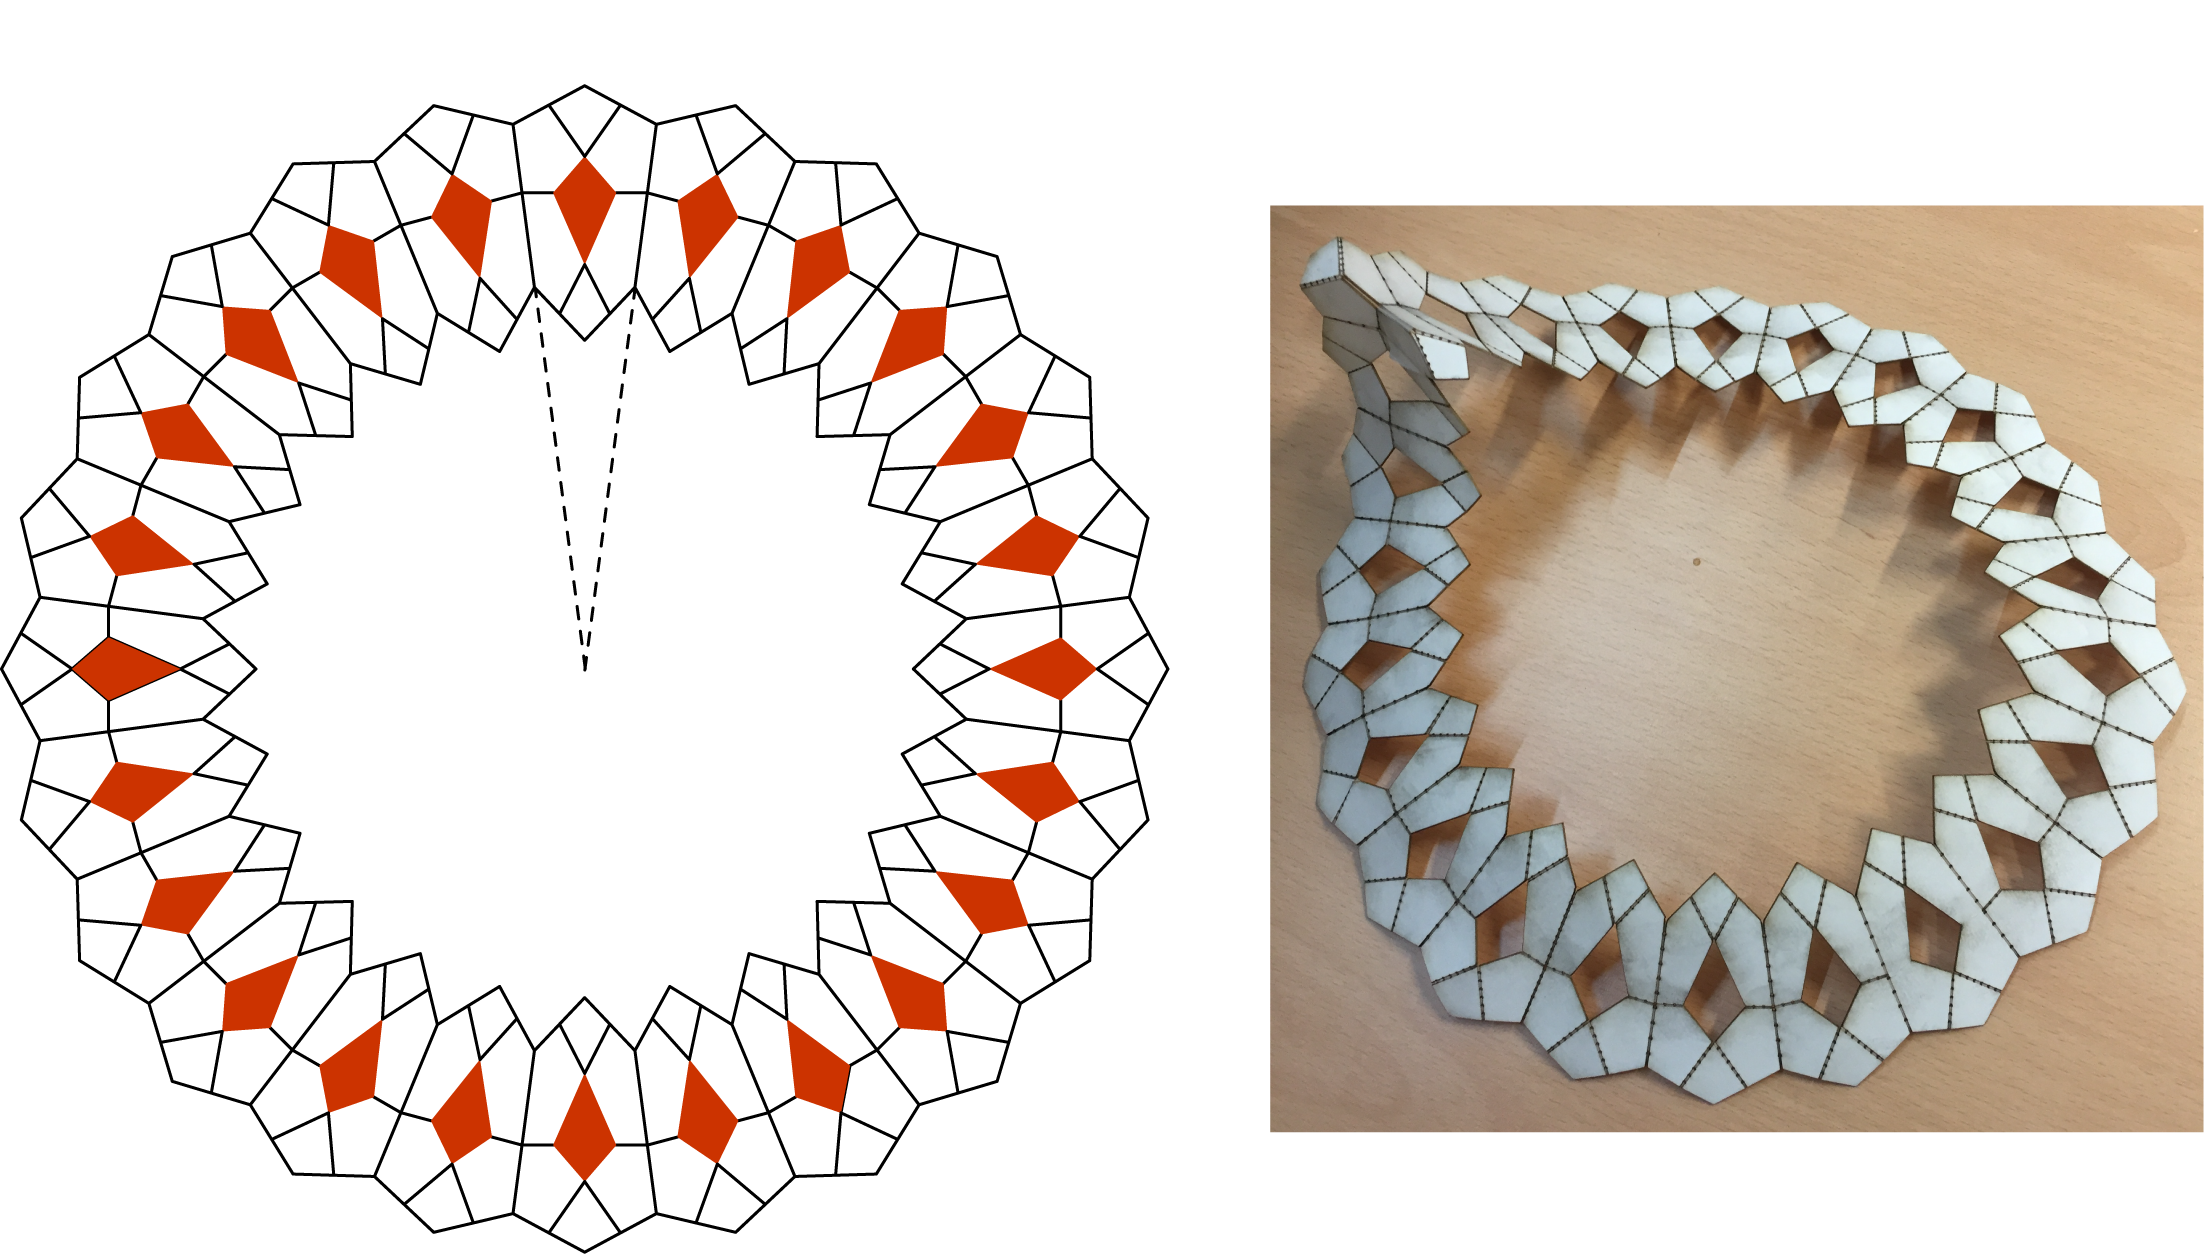
\includegraphics[width=.5\textwidth]{hexring24.png}
\end{center}
\caption{A 1D tessellation of singly-symmetric hexagonal cells. This cell can be used to create conical forms.}
\label{hexring} 
\end{figure}
%
Thus, we can developed a tessellating kirigami unit cell that, through geometry prescription, can take a variety of forms while obeying a single kinematic relationship. We can imagine manufacturing many of these cells for use in deployable sheets where curvature is required. Utilizing the parameterizations here, designs can be exactly calculated to achieve arbitrary, singly curved shapes. We can use both rigid folding techniques and create designs with a known amount of compliance depending on the symmetry of the desired structure. 

\end{document}
